\chapter{Solución con sensores IMU\label{sec:IMU}}
%------------------------------
%------___SOLUCIÓN_IMU___------
%------------------------------

\textcolor{rositaoscuro}{asdf}
\textcolor{teal}{sdffsd}

\label{sec:IMU4}

%--Marco conceptual
\section{Marco conceptual}
\label{sec:marco4}

Este apartado tiene por finalidad realizar una clara exposición de los conceptos teóricos fundamentales para la comprensión del diseño llevado a cabo. 


%--asdf
\subsection{asdf}
\label{sec:asdf4}


%--Desarrollo del prototipo
\section{Desarrollo del prototipo}
\label{sec:prototipo4}

\subsection{Materiales}
\label{sec:materiales4}


\subsection{Proceso de fabricación del soporte físico}
\label{sec:proceso4}
%Elaboración

\subsection{Funcionamiento}
\label{sec:funcionamiento4}
asdf



\section{Resultados y análisis}
\label{sec:resultados4}





\section{---------------}


\section{Sensores inerciales}
\subsection{Principio de funcionamiento}

Un sistema de referencia inercial se trata de un sistema de referencia regido por las leyes de movimiento de Newton. Por tanto, un sensor capaz de medir valores respecto a dicho sistema de referencia es lo que se conoce como un sensor inercial.

Una unidad inercial o IMU (Inertial Magnetic Unit) es un dispositivo que se compone de tres giróscopos (para determinar la orientación), tres acelerómetros y un reloj que permite asignar tiempo a los valores medidos por los sensores inerciales. Dichas unidades inerciales presentan tres ejes y cada uno de ellos presenta un acelerómetro y un giróscopo.

Por tanto, la información que se recoge de las unidades inerciales son aceleraciones lineales, velocidades angulares y tiempo común para los tres ejes que llevan dicha información de aceleración y velocidad angular (ver Figura \ref{fig:Imu}). 


El tiempo requerido para la implementación del sistema de medida puede influir en la marcha de los pacientes y por tanto en la obtención de los parámetros \cite{begona}. Los sensores inerciales utilizados permiten realizar las mediciones de una manera sencilla y rápida lo cual resulta beneficioso en el contexto ambulatorio tanto para los pacientes como para el personal sanitario



\subsection{Sensores inerciales propuestos}
Los sensores inerciales utilizados para el sistema son el modelo MTw Awinda (Xsens Technologies B.V, The Netherlands) pueden verse representados en la Figura \ref{fig:sensor_XSENS}



Su tamaño es de 47 x 30 x 13mm y 16g de peso por lo que puede definirse como un sistema compacto y ergonómico que será de utilidad para el sistema propuesto en este trabajo. Dispone de unas bandas de sujeción que permiten colocar el sensor en el lugar necesario y por tanto dota de versatilidad al diseño. 

Además, se incluye un software de captura que resultará útil para obtener las señales para su posterior procesado. La comunicación de los sensores con el software emplea un protocolo propietario que aparece representado en la Figura \ref{fig:protocolo}.

\subsubsection{Sensores inerciales}

	
	Para la obtención del dato de distancia a partir de las señales proporcionados por los sensores inerciales es necesario tener en cuenta que la distancia se recorre en el plano en el que se produce el avance, que es este caso es el plano XY.

Para obtener la posición en este plano a partir de la aceleración en los tres ejes XYZ proporcionada por los sensores inerciales, es necesaria una doble integración.Posteriormente se elimina la deriva existente en las señales debido a esta integración. A continuación se describen los cálculos realizados

Una vez calculadas las distancias necesarias, se procede al cálculo de la distancia de separación entre pasos. En la Figura \ref{fig:sep} se representa dicho cálculo. La distancia D2 es la correspondiente al cálculo de la distancia con el sensor inercial izquierdo en este caso, la distancia D1 es la distancia calculada mediante el sensor de ultrasonido.
\begin{figure}[H]
	\centering
	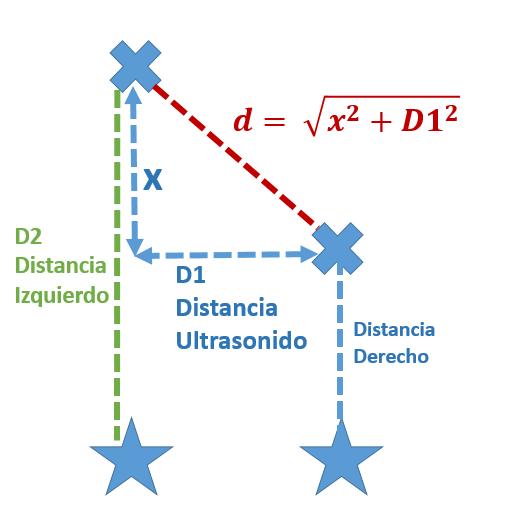
\includegraphics[width=0.8\textwidth]{./graphics/sep}
	\caption{Cálculo final de distancia de separación entre pasos} \label{fig:sep}
\end{figure}

Por tanto, para obtener X se utiliza la ecuación \ref{eq:x}
\begin{equation}\label{eq:x}
x = D2 - DistanciaDerecho
\end{equation}
En el caso de que el primero de los pasos se comenzase con el izquierdo la ecuación es la relativa a la DistanciaIzquierdo.

Para determinar la distancia, se utiliza por tanto, la ecuación \ref{eq:d}
\begin{equation}\label{eq:d}
d = \sqrt{x^{2}+D1^{2}}
\end{equation}